\section{New common privacy weaknesses} \label{sec:cwe-proposal}

Our study has shown the gaps in the existing CWE and CVE systems in terms of covering privacy vulnerabilities. To fill these gaps, we propose 11 new common privacy weaknesses to be added to the CWE system. We focus on CWE instead of CVE since CVE specifies unique vulnerabilities existing in specific software systems and application, while CWEs are at the generic level, similar to our taxonomy of privacy threats. We followed the CWE schema \cite{CWEschema2021} to define the new CWE entries which include attributes such as name, description, mode of introduction, common consequence, detection method, potential mitigation and demonstrative example. These attributes provide an overview of a privacy weakness in terms of its causes and consequences, and mitigation methods.

\newtext{Security vulnerabilities can typically be well specified as concrete hardware/software attacks that can be exploited to bypass the system's security. Unlike security vulnerabilities, privacy vulnerabilities seem to be more contextual than security vulnerabilities and its operationalisation may differ depending on context. In our study, we tried to formalise the privacy vulnerabilities as software attacks that are harmful to personal data and violate individual rights. Thus, it is important to provide the detailed description in each attribute in the identified 11 common privacy weaknesses since it defines a specific scenario that potentially leads privacy vulnerabilities.}

The proposed common privacy weaknesses address four groups of threats: surveillance, insecurity, secondary use and exclusion. The weaknesses in the insecurity group can be detected and resolved by implementing security mechanisms to better protect personal data and user privacy. On the other hand, the other groups of weaknesses require more attention from software development teams on examining privacy constraints involved, and designing relevant functions to respond to those constraints. The software development team needs to determine relevant functions, take privacy constraints into consideration and regularly review existing functions to ensure that they do not violate user privacy. For example, a user may want to change his/her user preferences when a new feature is launched, or a system must notify its users when there is a change to the policy that they have given consent to.

Due to space limit, we present here two examples (see Table \ref{tab:cwe-template-missing-consent-withdrawal} and Table \ref{tab:cwe-template-missing-consent-check}) of the new CWE privacy weaknesses and refer to the readers to our replication package \cite{rep-pkg-privul} for the remaining newly proposed CWEs. Table \ref{tab:cwe-template-missing-consent-withdrawal} shows a new common privacy weakness for not allowing a user to withdraw his/her consent. This weakness belongs to the exclusion category. Following the CWE schema, a short summary of the weakness is provided in its name, while a detailed description is provided in the description section. The mode of introduction briefly discusses how and when the weakness is introduced, which in this case is the architecture and design phase.

\begin{table}[ht]
	\centering
	\caption{An example of a missing consent withdrawal weakness.}
	\label{tab:cwe-template-missing-consent-withdrawal}
	\begin{tabular}{|p{8.5cm}|}
		\hline
		\textbf{Subcategory:} Exclusion \\
		\textbf{Class:} Not allowing a user to withdraw his/her consent \\
		\textbf{Name:} Missing consent withdrawal  \\
		\textbf{Description:} The software forces users to give consent before providing its services. These services may include personal data processing. However, the software does not a provide a function for users to withdraw their consent. The users can only accept consent, but they cannot withdraw their consent when they wish to. This vulnerability seriously violates user privacy. \\
		\textbf{Mode of introduction:} Phase: Architecture and Design. This weakness is caused by a missing privacy consideration about consent management and its related processes, which leads to the missing consent withdrawal function. \\
		\textbf{Common consequence:} The software violates user privacy by not allowing users to express their agreement on the use of their personal data. \\
		\textbf{Detection method:} Method: Manual analysis. Description: A consent management page or window in a software does not show an icon or option to withdraw consent. \\
		\textbf{Potential mitigations:} Phase: Architecture and Design. Strategy: User consent withdrawal consideration. Description: The software development team should consider which points in the software that should provide a user an ability to withdraw consent. \\
		\textbf{Demonstrative example:} Issue MDL-62309 in Moodle reports that the users cannot withdraw consent and cannot enter the site without giving consent. This issue violates user privacy as the users should be able to freely withdraw consent. \\
		\hline
	\end{tabular}
\end{table}

\begin{figure}[ht]
	\centering
	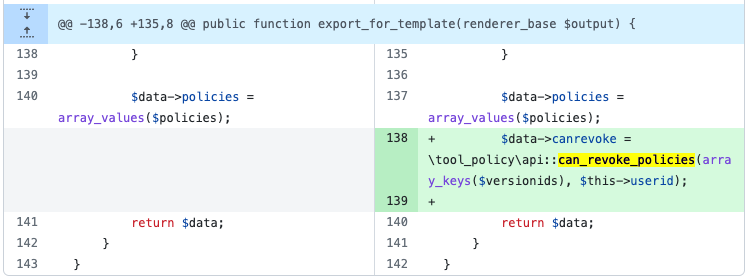
\includegraphics[width=1.0\linewidth]{figures/mdl-missing-consent-withdrawal}
	\caption{An example of missing consent withdrawal function in Moodle (Issue MDL-62309).}
	\label{fig:mdl-missing-consent-withdrawal}
\end{figure}

\begin{table}[ht]
	\centering
	\caption{An example of a collecting personal data without user consent/permissions weakness.}
	\label{tab:cwe-template-missing-consent-check}
	\begin{tabular}{|p{8.5cm}|}
		\hline
		\textbf{Subcategory:} Surveillance \\
		\textbf{Class:} Collecting personal data without user consent/permissions \\
		\textbf{Name:} Missing a consent check before collecting personal data \\
		\textbf{Description:} The software does not check for a user consent prior to personal data collection. This makes the software collect personal data that users have not given consent to (e.g., location and speech). \\
		\textbf{Mode of introduction:} Phase: Implementation. This weakness is caused by missing a consent check before collecting personal data. \\
		\textbf{Common consequence:} The software violates user privacy since users has not given consent/permissions to collect their personal data. \\
		\textbf{Detection method:} Method: Manual analysis. Description: Perform a code check at points of personal data collection. \\
		\textbf{Potential mitigations:} Phase: Implementation. Strategy: Check for user consent before collecting data. Description: The software development team should perform a consent check at every point that collects personal data in the software. \\
		\textbf{Demonstrative example:} A commit 0b09df0 in HumanDynamics repository collects user speech without consent check. \\
		\hline
	\end{tabular}
\end{table}

\begin{figure}[ht]
	\centering
	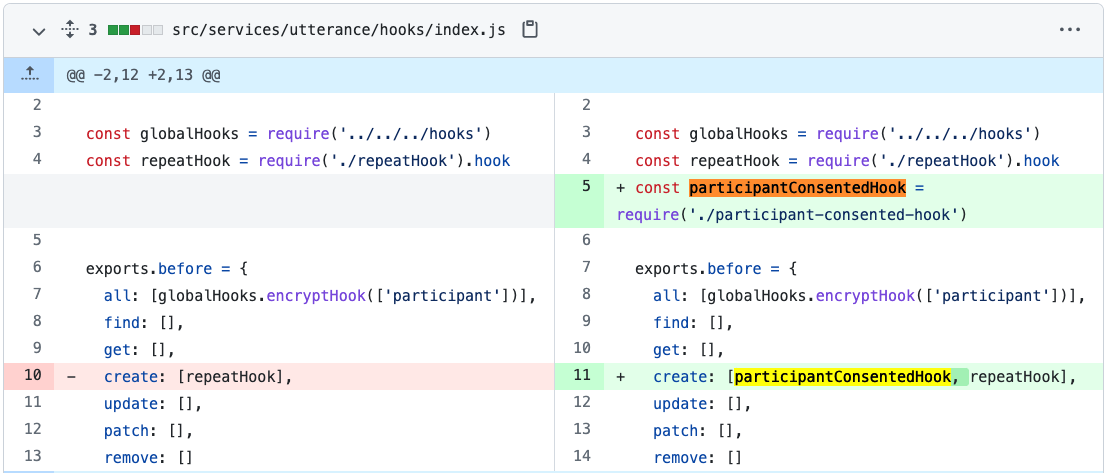
\includegraphics[width=1.0\linewidth]{figures/hd-missing-consent-check}
	\caption{An example of missing a consent check before collecting personal data in HumanDynamics (Commit 0b09df0).}
	\label{fig:hd-missing-consent-check}
\end{figure}

The common consequence section identifies a privacy property that is violated and an effect that is caused by the weakness. The detection method section describes different methods that the weakness can be detected in software. We also propose methods to mitigate the weakness. It is noted that different phases in software development may pose different privacy concerns. Finally, we provide a demonstrative example of the new weaknesses by extracting code fragments, issue reports and commits from real software repositories hosted on GitHub\footnote{\url{https://github.com/}}. \newtext{We used the keywords in the weakness class and name to search for relevant code, commits and issues. Once the search results were returned from GitHub, we went through the descriptions and identified the demonstrative example from those results.} For example, Figure \ref{fig:mdl-missing-consent-withdrawal} shows a code fragment extracted from the Github commit \emph{ad5e213}\footnote{\url{https://github.com/moodle/moodle/commit/ad5e213}} in Issue MDL-62309\footnote{https://tracker.moodle.org/browse/MDL-62309} of the Moodle project. This example demonstrates the existence of the missing consent withdrawal weakness in practice.

Table \ref{tab:cwe-template-missing-consent-check} presents a new common privacy weakness for collecting personal data without user consent/permissions. This weakness belongs to improper personal data collection category. Figure \ref{fig:hd-missing-consent-check} shows a code fragment confirming the existence of a missing consent check before collecting personal data weakness. The code fragment is extracted from the Github commit \emph{0b09df0}\footnote{\url{https://github.com/HumanDynamics/rhythm-server/commit/0b09df0}} in the HumanDynamic repository \cite{HumanDynamics}.

\begin{conclusion}
	\textbf{We propose 11 new common privacy weaknesses to be added to CWE. These will significantly improve the coverage of privacy weaknesses and vulnerabilities in CWE, and subsequently CVE.}
\end{conclusion}
